\documentclass{article}
\usepackage[utf8]{inputenc}
\usepackage{graphicx}
\usepackage{fancyhdr}
\usepackage{geometry}
\usepackage{amsmath}
\usepackage{amssymb}
\usepackage{url}
\usepackage{hyperref}
\usepackage{subcaption}

\geometry{left = 2.5cm, right=2.5cm, bottom=2.5cm, top=2.5cm}

\title{3806ICT - Assignment 1}
\author{Nick van der Merwe - s5151332 - nick.vandermerwe@griffithuni.edu.au}

\pagestyle{fancy}
\renewcommand{\headrulewidth}{1pt}
\fancyhf{}
\rhead{3806ICT - Assignment 1}
\chead{Griffith University}
\lhead{Nick van der Merwe - s5151332}
\rfoot{Page \thepage}
\newcommand\tab[1][1cm]{\hspace*{#1}}

\begin{document}
\maketitle
\section{Introduction}
In this piece a controller is defined for a robot using a proportional integral
derivative controller. This is split into two tasks, defining the PID algorithm
and the Kalman filter in the assignment. However, the architecture of the
solution will contain four parts: the sonar wrapper, the PID service, the Kalman
filter service and the controller. Essentially, the sonar wrapper will turn the
sonar topic into a service so that the controller does not subscribe to it. The
PID and the Kalman filter will be purely functions without any storage so that
they can be reused in the future. Lastly, the controller node will manage all of
the data. \\ 
\tab This report is organised based on the content in the nodes. Each section
will introduce the necessary theory and explain how that is converted into code.
With that in mind, Section \ref{sonarSection} contains the sonar wrapper,
Section \ref{pidSection} covers the PID equation (not defining the constants), 
Section \ref{kalmanSection} runs over the kalman filter (not finding the
variance), and Section \ref{controllerSection} defines the controller. The
controller contains how all the previous nodes are tied together, including how
the constants in PID are defined and variance is found for the Kalman filter.
\section{Sonar Wrapper Node}\label{sonarSection}
This is quite straight forwards as it only requires us to save the last
published value in a variable. As a design decision to avoid global variables it
was made as a class. The code is visible in Figure \ref{sonarSrv} and
\ref{sonarCode}. 
\begin{figure}[ht]
    \begin{subfigure}{.5\textwidth}
        \centering
        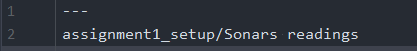
\includegraphics[scale=0.5]{img/sonar_wrapper_srv.png}
        \caption{}
        \label{sonarSrv}
    \end{subfigure}
    \begin{subfigure}{.5\textwidth}
        \centering
        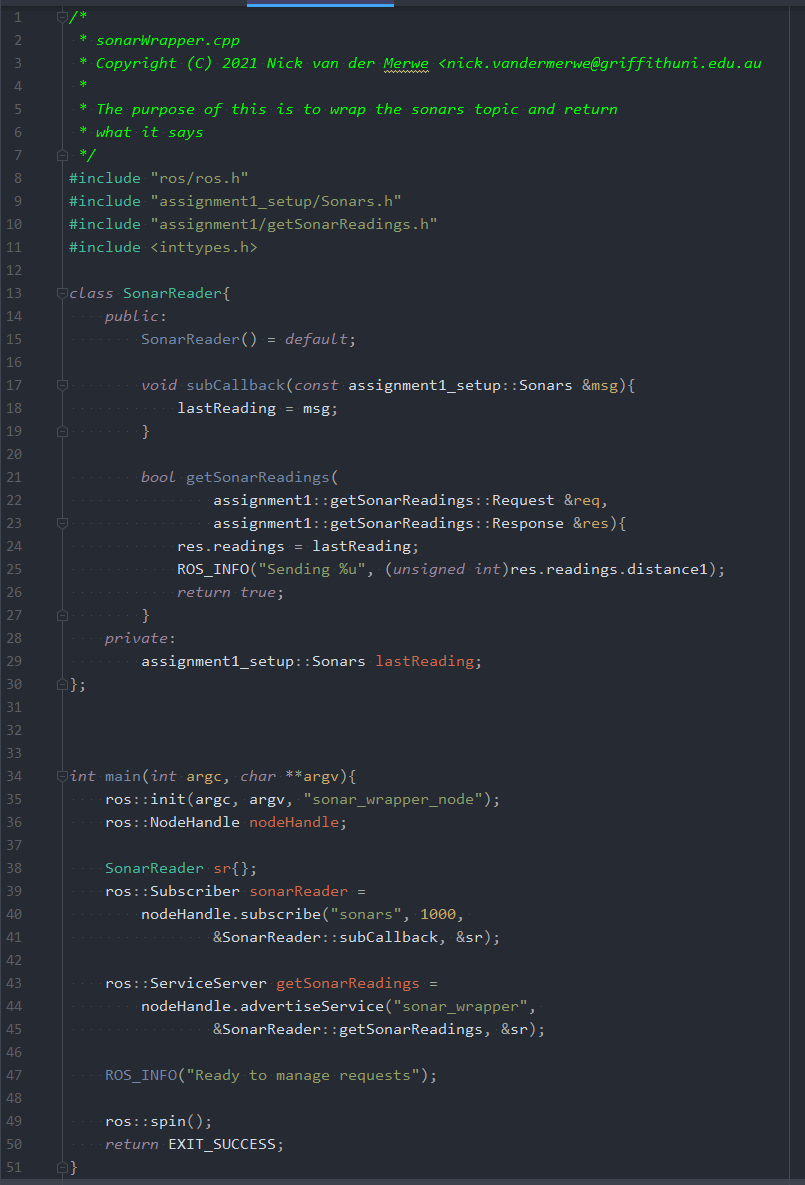
\includegraphics[scale=0.25]{img/sonar_wrapper.png}
        \caption{}
        \label{sonarCode}
    \end{subfigure}
    \caption{Sonar wrapper srv in a and code in b}
    \label{sonarWrapper}
\end{figure}

\newpage
\section{Task 1: PID Node}\label{pidSection}
Before the coding section, the mathematics behind what a proportional integral
derivative controller does must be explained. In short, the goal of the
controller is to minimise the error that is reported. As stated in the task, the
formula to be used here is in Equation \ref{pidEquation}.
\begin{equation}
    \label{pidEquation}
    \begin{split}
    Y(t) & = K_{p}e(t) + 
           K_{d}\frac{de(t)}{dt} +
           K_{i}\int^{t}_{0}e(t')dt' \\
    & = P(t) + D(t) + I(t)
    \end{split}
\end{equation}
\tab Where $e(t)$ is the input error: in our case the distance from the bowl.
$t$ is the time, $K_p$ is proportional gain, $K_d$ is the derivative gain and
$K_i$ is the integral gain. \\ \\
To make elaborating how this equation functions simpler, the first thing to
do is to consider each of the terms separately as they each represent a part of
\textbf{P}roportional \textbf{I}ntegral \textbf{D}erivative. To summarise, the
proportional section represents the current error, the integral is the error in the
past and the derivative is a prediction of the error into the future
\cite{pidControl}. The logic behind this is that for the P term its just the
current error, the integral is the area under the curve in the past and the
derivative is the change at that specific point.
These are each adjusted to the environment by using the K
terms on each term.  \\ \\
Now the next issue is that this representation uses continuous time whereas in
computational mathematics everything must be discrete - in this case our sonar
only reports every 10ms. The exact maths for converting this into discrete
values was covered in the lab content so it will not be copied over here, but
rather explained. \\
\tab The first step is to define time as discrete by making $T=10ms$ and 
$t_i = T+t_i-1$. Technically this would be all that's necessary, but the exact
way to calculate the derivative and integral is not known. For these the
conceptual meanings can be used: a derivative is the change in the 
output of a function in the smallest unit of time and an integral is the area
under the curve from one time to another. Another fact is that technically a
derivative forwards (current minus future) is the same as backwards (current
minus last value) in continuous time due to it being infinitely small. \\
\tab To take this and define them discretely with logic is simple. A derivative
is its current value subtracted by its last value, all divided by T (since that
is the smallest unit of time we have). Next the integral is simply the sum of
all the previous error values times T. This can conceptually be seen as how the
area of a square is found at a low level without multiplication: split it into
strips of size 1 (in our case T) and add these areas together. Including the K
terms, our equations are in Equations \ref{pTerm}, \ref{dTerm} and \ref{iTerm}.
\begin{equation}
    \label{pTerm}
    P(t) = K_{p}e(t) 
\end{equation}
\begin{equation}
    \label{dTerm}
    D(t) = K_{d} \frac{e(t_i) - e(t_{i-1})}{T}
\end{equation}
\begin{equation}
    \label{iTerm}
    I(t_i) = K_i \sum_{i=1}^i{Te(t_i)}
\end{equation}
Programmatically, it would be inefficient to do the integral by summing up
everything in this manner every time it is calculated, so realistically the
value is simply returned on its own in the function so that it can just be added
to once in the next run. This is represented as Equation \ref{iTermProper}.
\begin{equation}
    \label{iTermProper}
    \begin{split}
    I(t_i) & = K_{i}f(t) \\
    f(t) & = e(t_i)T + f(t_{i-1})
    \end{split}
\end{equation}
\newpage
The PID srv file and C++ code is visible in figure \ref{pidCode}.
\begin{figure}[ht]
    \centering
    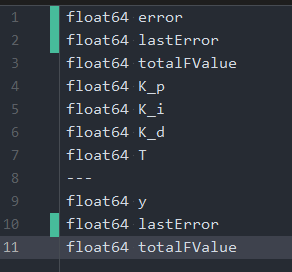
\includegraphics[scale=0.43]{img/pidSrv.png} \\
    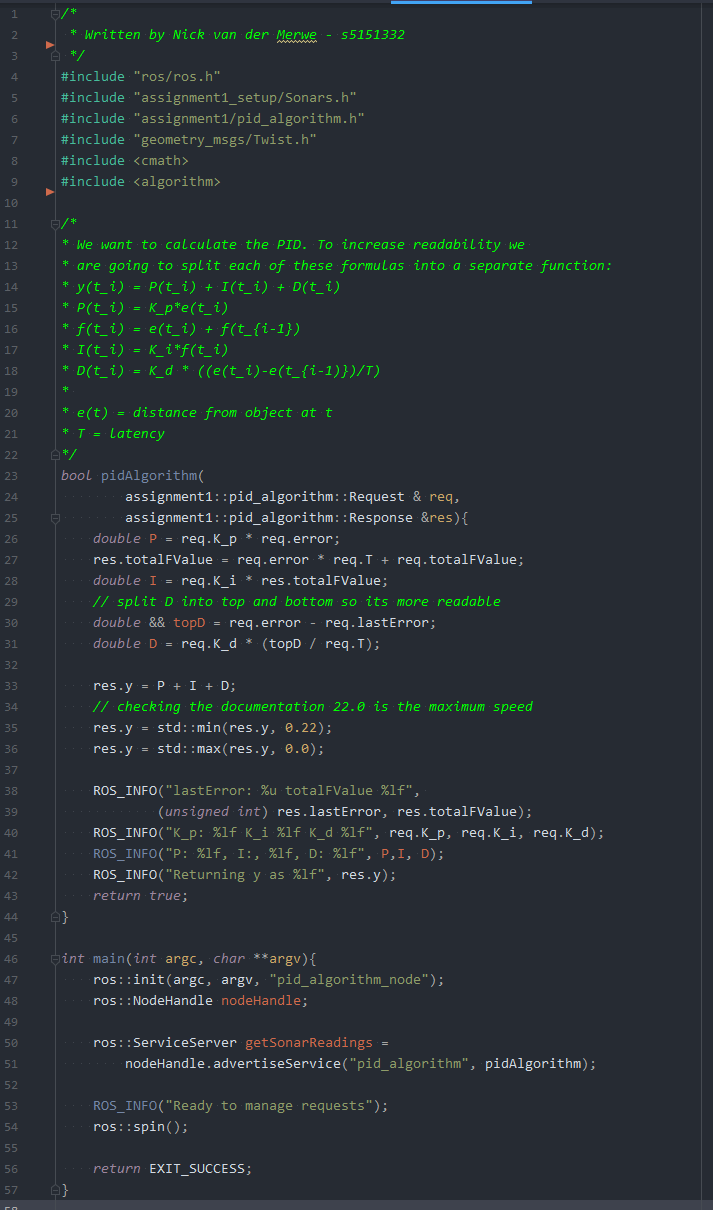
\includegraphics[scale=0.43]{img/pidAlgorithm.png}
    \caption{The PID srv and cpp files respectively}
    \label{pidCode}
\end{figure}
\newpage
\section{Task 2: Kalman Filter Node}\label{kalmanSection}
The goal of a Kalman filter is to get rid of noise in sonar readings through
maths, and in this case odometry readings. The equations to be used are defined
in Equations \ref{kalmanEquations}.
\begin{equation}
    \label{kalmanEquations}
    \begin{split}
        K_i & = \frac{P_i^-}{P_i^- + R_i} \\
        y_i & = y_i^- + K_i(z_i - y_i^-) \\
        P_{i} & = (1-K_i)P_i^-
    \end{split}
\end{equation}
Where $z_i$ is the sonar's reading, $y_i^-$ is the estimation of how far the
robot is from the bowl at step $i$, $P_i^-$ is the predicted variance at $i$,
and $R_i$ is the initial variance read. Since there are no continuous variables
in this, there is no need for this to be changed such as the PID. However, each
of these should still be properly explained.

\tab The naive way to solve the issue of a normally distributed noisy sonar
would simply be to measure the median every time. However, to do that the robot
would have to sit there for several seconds, move forwards slightly then sit
there and measure the median again. Instead, what the Kalman filter aims to do is
take the measuring once, move, (in our case) consider how far it moved through
the odometry, apply the Kalman filter to this and get an estimate of how far it
is \cite{kalman}. The reason why the odometry alone would not be enough is visible in how the
sonar functions. Consider the case where the bowl lies 13 degrees to the right
of the way the robot is facing. If we only use the euclidean distance measured
by the odometry system, it would not actually be the distance from the bowl.
From all of this, we can see the need for why the Kalman filter is necessary.

\tab For now the focus is on applying the Kalman filter step out of the steps
detailed previously which is all in equation \ref{kalmanEquations}. In short,
the goal of this step is to give readings varying weight depending on the
certainty of them. This weight is given by the Kalman gain by taking the
predicted variance divided by itself added to the overall variance. Then we can
add the difference in the reading and the estimated position to its estimated
position to find $y_i$. To calculate the next predicted variance is typically
complicated, but was compressed into multiplying $P_i^-$ by the complement of
the Kalman gain $(1-K_i)$. In practice this just makes later readings have less
weight.

\tab In an attempt to understand this particular equation, an interesting proof
by induction was found that makes calculating the variance irrelevant.
Essentially it's possible to remove $P_i$,  $P_i^-$ and $R_i$ from the
equations. First, let's change the notation so that the pattern is more obvious.
\begin{equation*}
    \begin{split}
        K_i = \frac{P_i}{P_i + R} \\
        P_{i+1} = (1-K_i)P_i \\
        P_0 = R
    \end{split}
\end{equation*}
First we define our base case of $K_0$
\begin{equation*}
    \begin{split}
        K_0 = \frac{P_0}{P_0 + R} \\
        P_0 = R \\
        K_0 = \frac{P_0}{2P_0} \\
        K_0 = \frac{1}{2}
    \end{split}
\end{equation*}
Now in induction we just have to prove the $i+1$ case
\begin{equation*}
    \begin{split}
        P_{i+1} & = R(1-K_i) \\
        K_{i+1} & = \frac{P_{i+1}}{P_{i+1} + R} \\
         & = \frac{R(1-K_i)}{R(1-K_i)+R} \\
         & = \frac{R(1-K_i)}{R-RK_i+R} \\
         & = \frac{R(1-K_i)}{2R - RK_i} \\
         & = \frac{R(1-K_i)}{R(2-K_i)} \\
         & = \frac{1-K_i}{2-K_i}
    \end{split}
\end{equation*}
So essentially we found that
\begin{equation*}
    \begin{split}
        K_0 & = \frac{1}{2} \\
        & = \frac{1-K_i}{2-K_i}
    \end{split}
\end{equation*}
\tab With this being said, it will just be ignored. It's an interesting proof that
makes variance useless, but taking it out will probably remove a section of the
assignment that the assignment writer intended the student to do. It's
essentially just evidence of extensive research around understanding the formulas
at work.
\\ \\
Moving onto the implementation, its a service that uses the exact formulas on
the task sheet visible in figure \ref{kalmanImplement}.
\begin{figure}[ht]
    \begin{subfigure}{.5\textwidth}
        \centering
        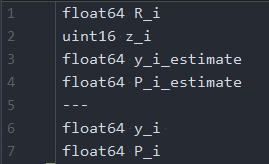
\includegraphics[scale=0.4]{img/kalman_filter_srv.png}
        \caption{}
        \label{kalmanSrv}
    \end{subfigure}
    \begin{subfigure}{.5\textwidth}
        \centering
        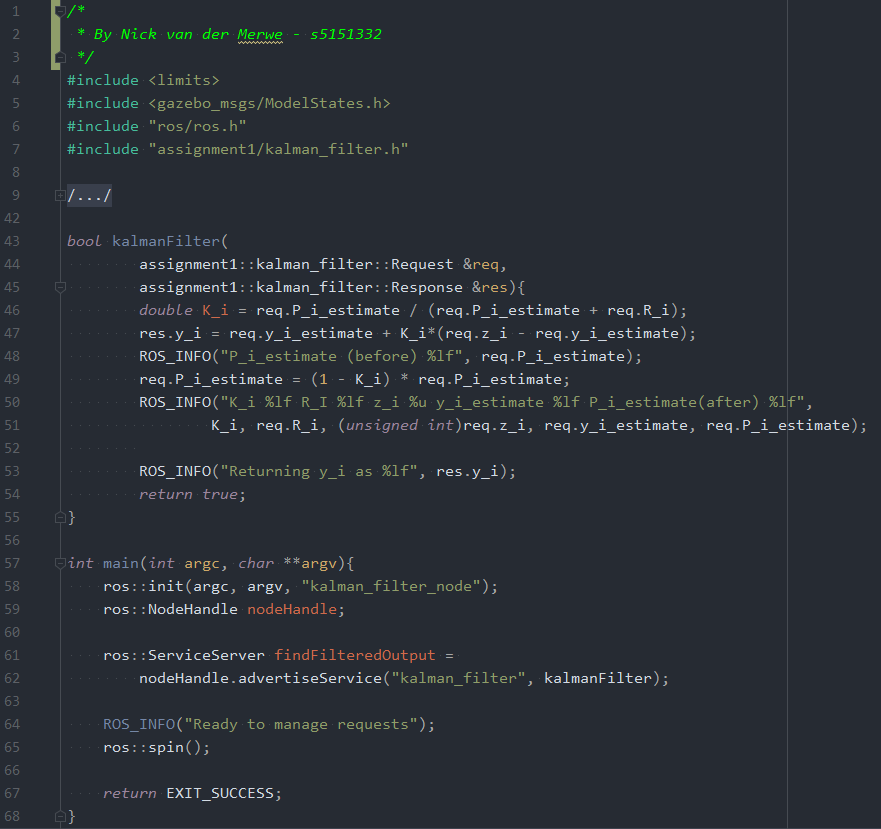
\includegraphics[scale=0.35]{img/kalman_filter.png}
        \caption{}
        \label{kalmanCode}
    \end{subfigure}
    \caption{Kalman filter implementation, srv file in \ref{kalmanSrv} and code
    in \ref{kalmanCode}}
    \label{kalmanImplement}
\end{figure}
\section{Controller Node}\label{controllerSection}
\subsection{PID constants}
As picking the PID terms is not an essential step and, only needs to be
justified, we can use manual selection. To define our PID terms we must consider
the goal of how we wish the robot to move. A reasonably logical approach would
be to make the robot run at maximum speed until it comes close to the bowl and
then slow down when its closer so that it can accurately move. To align this
with a real world goal, it's wanting to drive to a location as fast as possible
yet be safe. In other words, when a car is parking it slows down so it can move
more accurately.
\\
\tab The $K_p$ term does exactly this by changing its speed in respect to its
distance from the target. As such we can pick a point that looks reasonably
close (see figure \ref{100units}) and define that as the point it should start
slowing. To work out the $K_p$ from this all that must be done is the maximum
speed should be found when its at 100 units by doing $y(t)=K_pe(t) => 0.22 = K_p100 =>
K_p = 0.22/100$. 
\begin{figure}[ht]
    \centering
    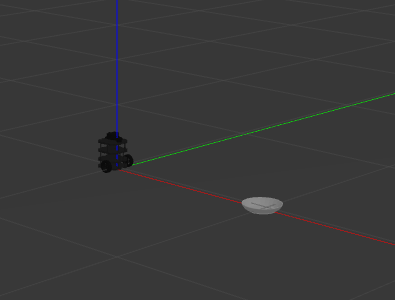
\includegraphics[scale=0.75]{img/100_units_away.png}
    \caption{How far the robot looks when it's 100 units away}
    \label{100units}
\end{figure}
\\
\tab One issue to consider is that typically the error in PID is not just
distance (i.e. its the difference between the goal speed and current speed),
which is especially impactful to the integral term. Usually when the 
error hits zero, the integral value is set as a constant - otherwise it would
continue to rise as the controller is running \cite{kalman}. In this case it only
occurs when the robot actually reaches the bowl - which would be the end of the
problem. In the case that the robot is as far away as its sonar readers allow
(around 60,000), it would likely mean that it will just run at maximum speed all
the way to the bowl. This results in three options: 1) Set $K_i$ to close to 0,
rendering the entire term next to useless 2) Let the robot just run at maximum speed
when its far away 3) Decide on a point when the integral term should stop
changing. \\ 
\tab To be true to the goal, the best option here would be option 1. Option 2 is
in direct conflict with the goal of slowing down when close as it renders it
impossible in some situations, and picking an arbitrary point where the integral
stops growing would only cause the robot to have a minimum constant speed after
a certain point. While $K_i$ could be set close to zero such that it has a
'conceptual' effect, it's easier to just set it to zero as it would affect the
speed in the same way in this environment.
\\ \\
As the derivative term allows the robot to continue going a certain speed
or slow down less than usual, it could be useful in the Kalman filter. This is
because occasionally the error is filtered to be a negative value which in that
case the P term completely stops, and often far too early. Furthermore, even
with just the P term on its own in a non-noisy sonar it starts going abysmally
slow as it approaches it. As a solution, $K_d$ is defined such that the robot
an only lose $80\%$ of its speed every second. To do this, the meaning of what
the D term should be understood fully. It takes in the current distance,
subtracts the last distance and divides by T. The subtraction operation, in
theory, should always lead to a negative number as we are approaching the goal
and dividing by T (0.01 seconds) says what the velocity would be for a second -
as a negative. From this all that must be done to make sure 20\% of the previous
velocity is added,$K_d$ should equal $-0.2$ as to cancel the negative and
represent its velocity every second.
\\
\tab In reality though, due to the factor that the sonar readings are integers
this does not function as intended. The maximum speed is 22 centimetres per
second, and its reporting that 100 times every second. In other words, every
four (or so) readings the difference would be 1cm, and not every reading has a
difference of 0.22. As a result, the D term simply adds four times more than the
intended value every four iterations. Since this is a sonar based issue, there
is not much of a work around other than turning the sonar reading into a
float64, ignoring the issue or setting $K_d$ to zero. Out of these, the issue was
chosen to be ignored as in the Kalman filter this is not what occurs: the
readings are floats.
\\ \\
To tie it together, it was decided that $K_p=0.22/100$, $K_i=0$, $K_d=-0.2$.
$K_p$ makes the robot slow down as it approaches and $K_d$ prevents the robot
from slowing down too abruptly. The issue with $K_i$ is that it makes the robot
either stay at a certain speed, or stay at maximum speed depending on how its
implemented.  
\subsection{Calculating Variance}
To do this is not any different from usual:
\begin{equation}
    \begin{split}
        mean & = \frac{1}{n} \sum_{i=0}^n{x_i} \\
        variance & = \frac{\sum_{i=0}^n{(x_i - mean)^2}}{n-1}
    \end{split}
\end{equation}
where $x_i$ is a collected sample and n is the number of samples
\cite{variance}. Note that the sample formula is used instead of the population
formula. With regards to the number of samples collected, it was decided that
1000 will be used. Realistically, this is hard to justify without other
variables involved but at 1000 points it is expected to give ten points for
every percentile which should be reasonable.  
\\ \tab One option is to hard-code in the variance because in the $sonars.cc$ 
source code provided $std::normal\_distribution()$ is used and the standard
deviation is defined as $100$. Meaning, the variance is hard-coded to $100^2 =
10,000$. However, hard-coding in the answer would destroy an intended part of
the assignment and reduce reusability in the case that the sonar reader's
distribution changes. Furthermore, this can be used as justification for why the
variance is calculated every run: to improve reusability.
\subsection{Random turns due to noise}
Due to the sonars being capable of randomly shooting to uint16's max (even if
the chance is low), it is possible for the robot to accidentally shift out of
sight of the bowl if one comes through. To counteract this, it was implemented
that the robot should read that it lost sight of the bowl five consecutive times
before it turns. While technically possible, the chances of this occurring is low
enough that it does not happen. 
\newpage
\subsection{Structure}
A core factor that makes implementing this difficult is that extracting functions
from main in ROS is often prohibited due to a couple of methods only being
permitted to be called inside main. So for easier understanding, figure
\ref{controllerPseudo} was made to grasp the implementation better. However, it
should only be used as a guide to the general structure - some extra things were
added in the code that was detailed in the justifications, but not the pseudo-code.
\begin{figure}[ht]
    \begin{subfigure}{.5\textwidth}
        \centering
        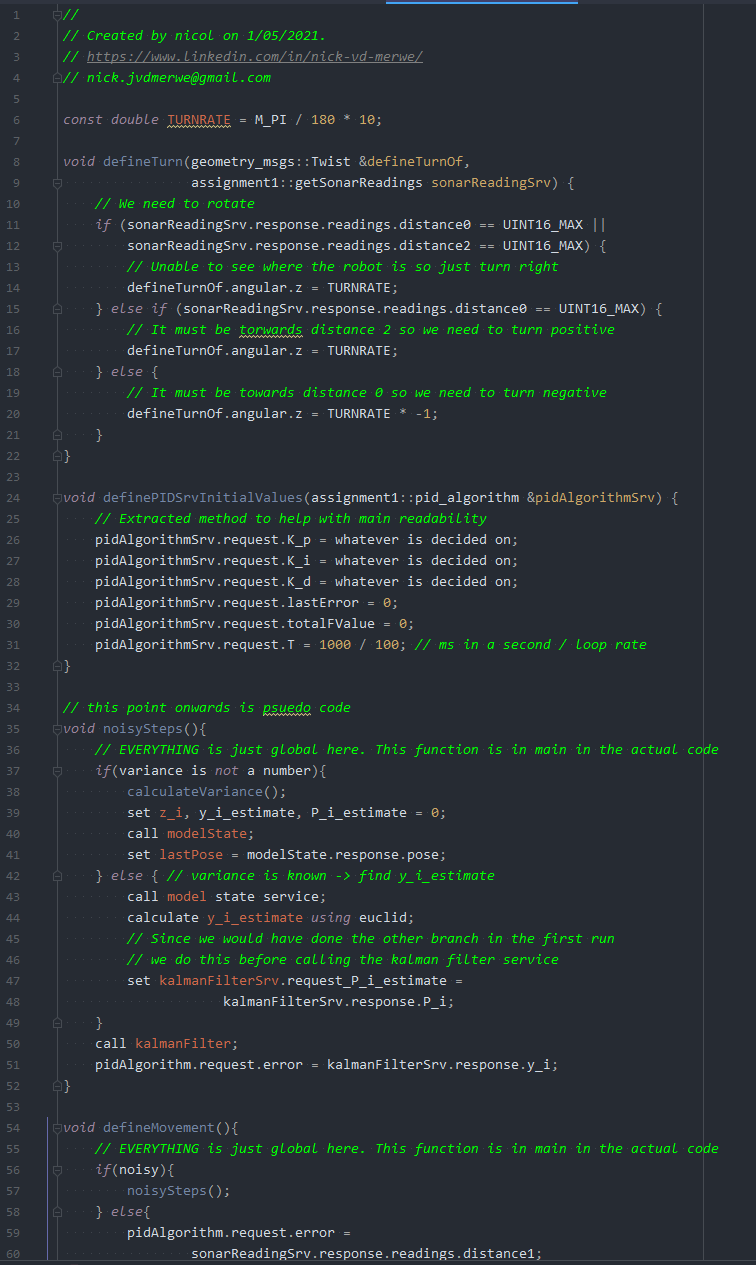
\includegraphics[scale=0.22]{img/pseudocode_1.png}
    \end{subfigure}
    \begin{subfigure}{.5\textwidth}
        \centering
        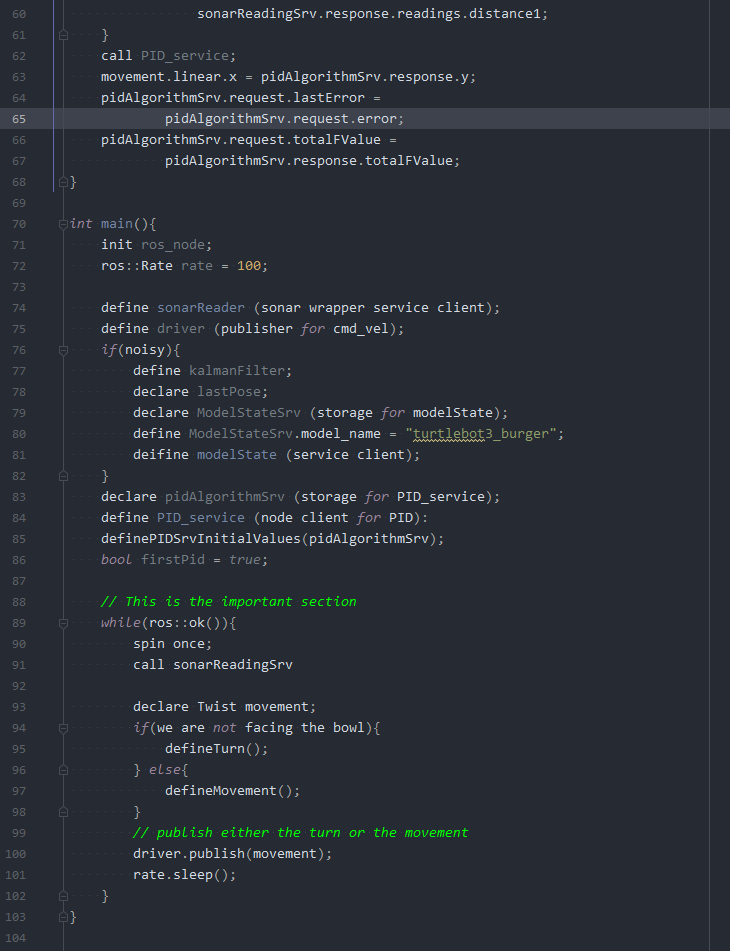
\includegraphics[scale=0.30]{img/pseudocode_2.png}
    \end{subfigure}
    \caption{Pseudocode for better understanding of main code}
    \label{controllerPseudo}
\end{figure}
\subsection{Implementation}
Following the pseudocode, the controller was implemented as visible in figure
\ref{controllerPseudo}. 
\begin{figure*}[ht]
    \begin{subfigure}{.5\textwidth}
        \centering
        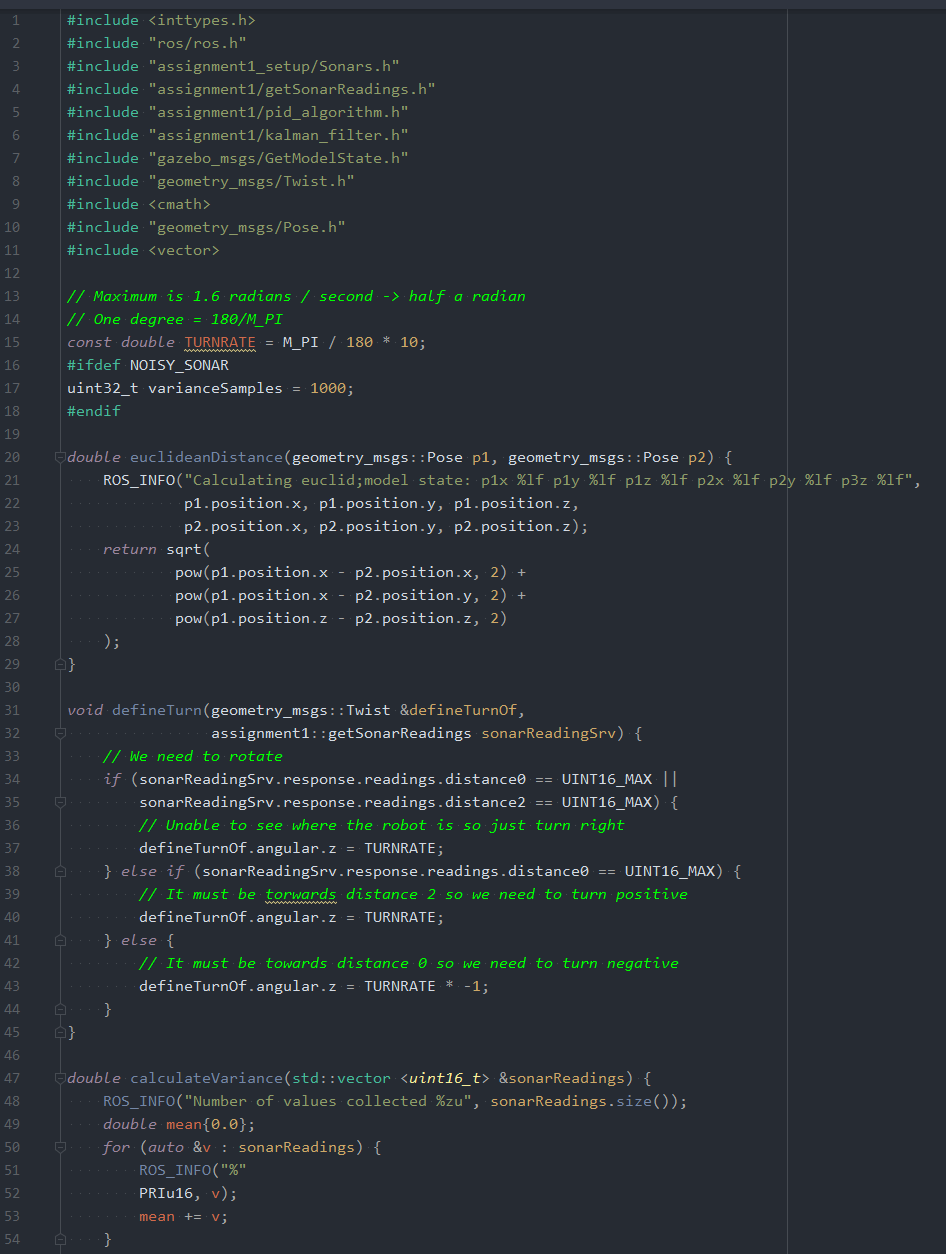
\includegraphics[scale=0.24]{img/controller1.png}
    \end{subfigure}
    \begin{subfigure}{.5\textwidth}
        \centering
        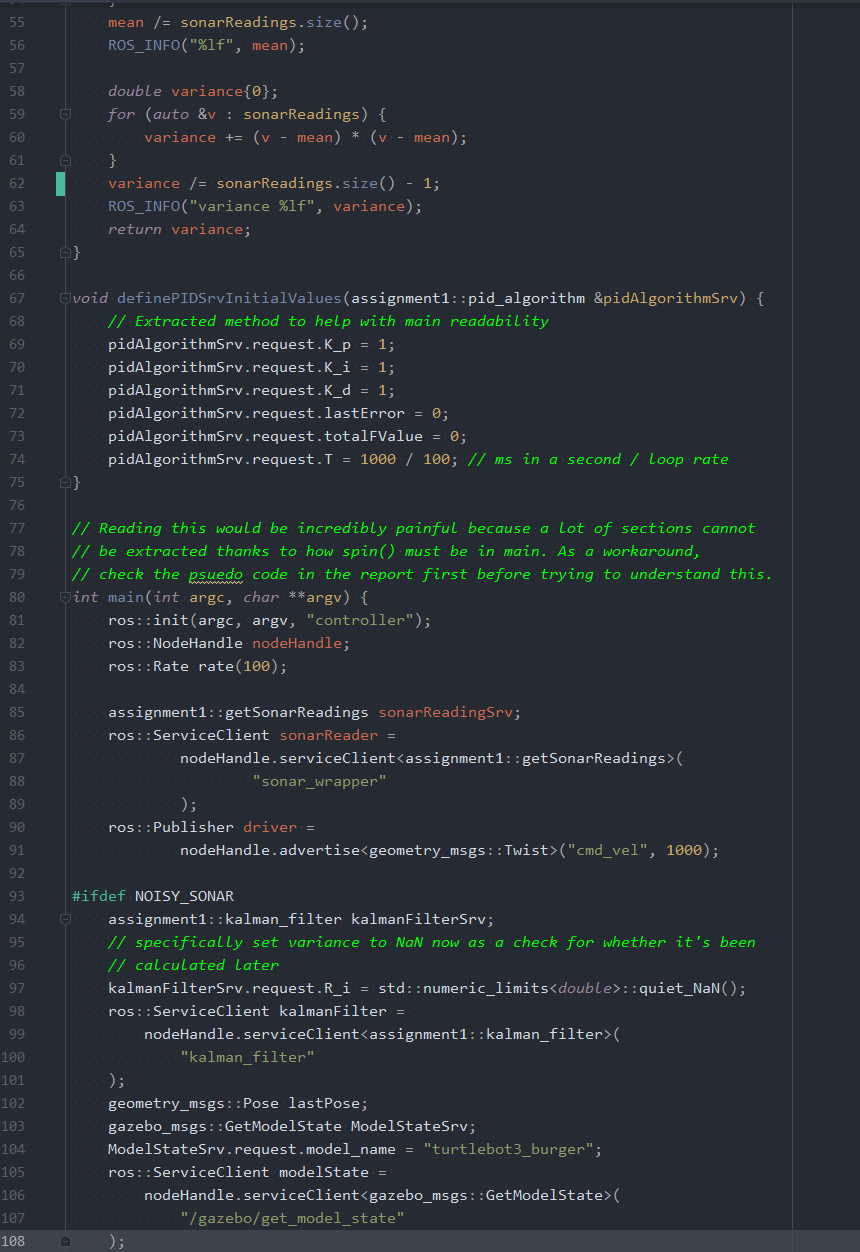
\includegraphics[scale=0.24]{img/controller2.png}
    \end{subfigure}
\end{figure*}
\begin{figure*}[ht]
    \begin{subfigure}{.5\textwidth}
        \centering
        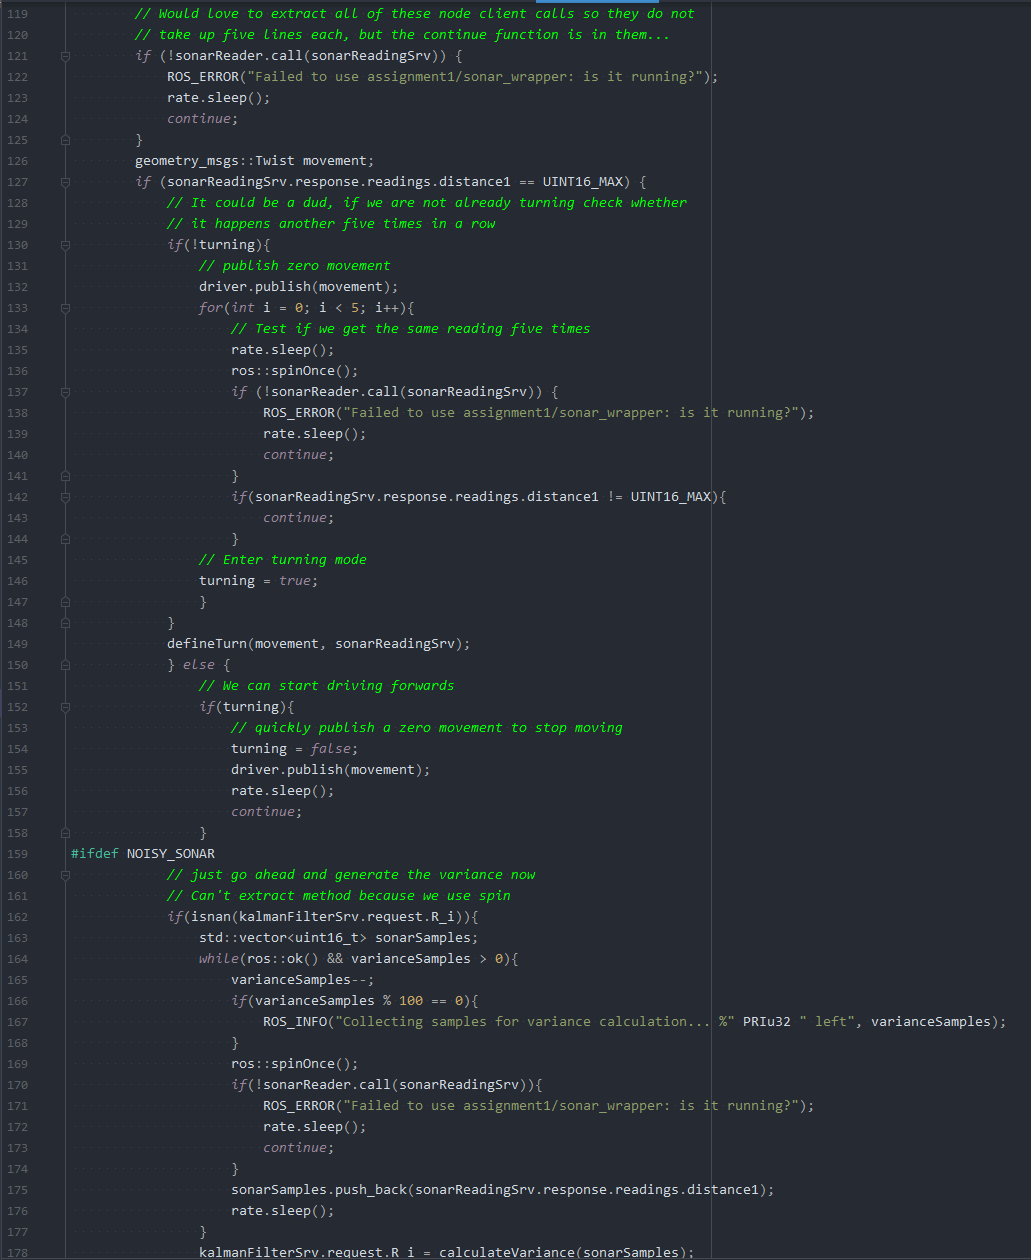
\includegraphics[scale=0.24]{img/controller3.png}
    \end{subfigure}
    \begin{subfigure}{.5\textwidth}
        \centering
        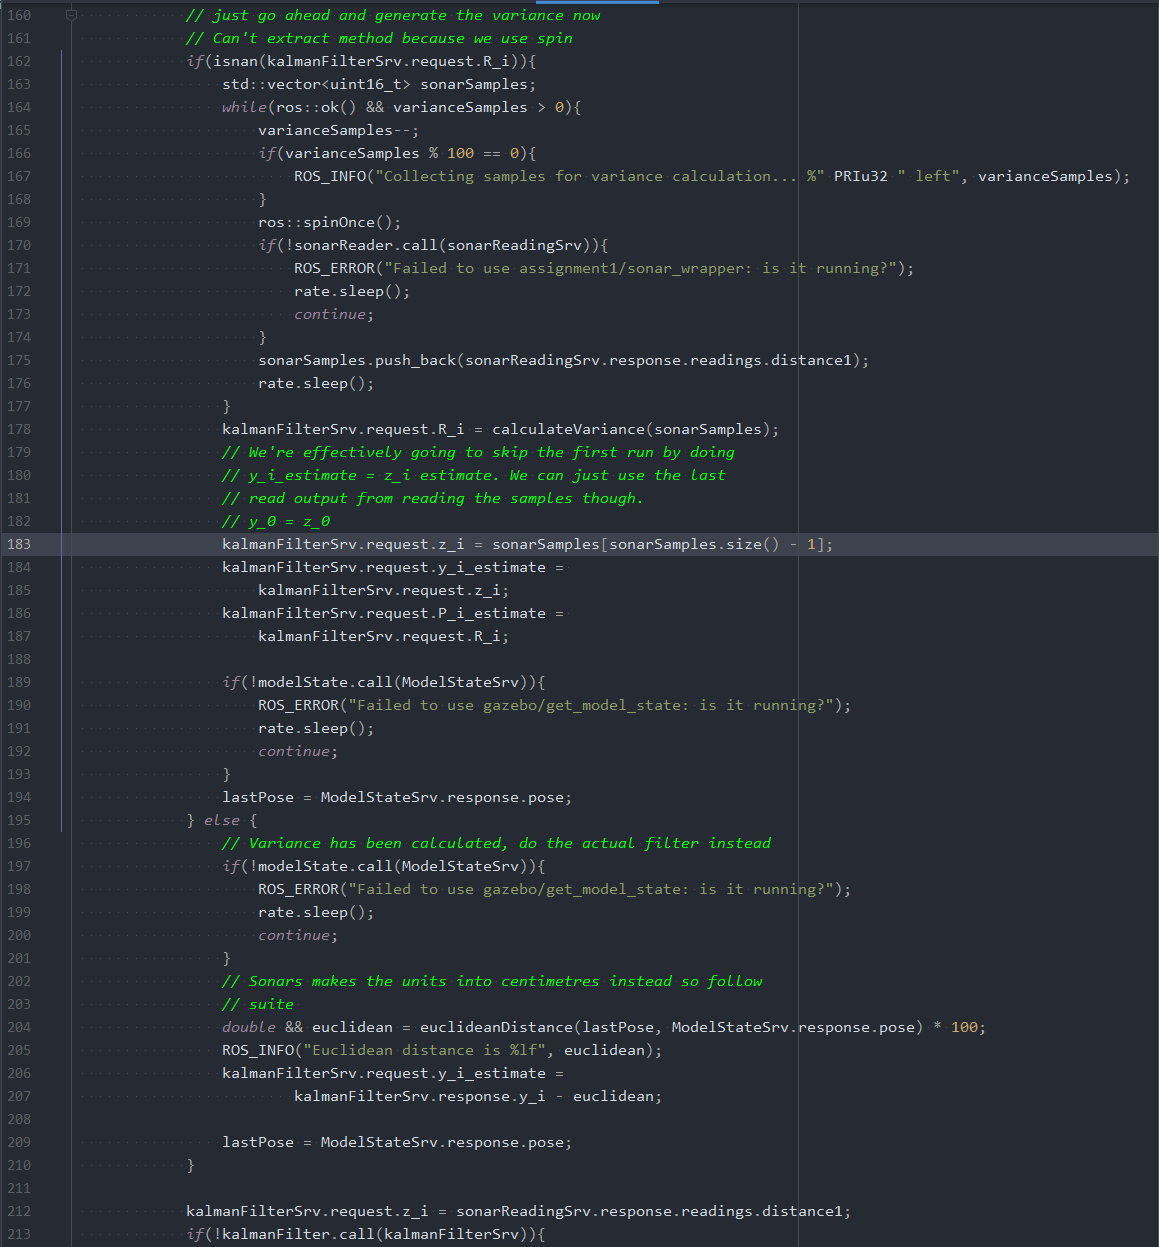
\includegraphics[scale=0.24]{img/controller4.png}
    \end{subfigure}
\end{figure*}
\newpage
\begin{figure}[ht]
    \centering
    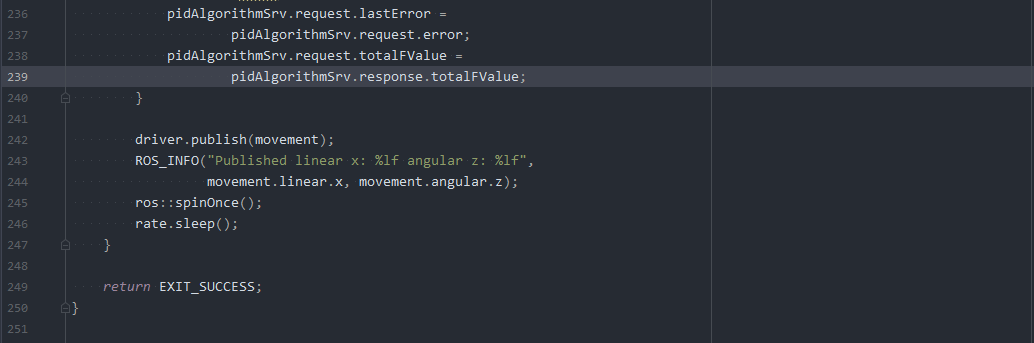
\includegraphics[scale=0.24]{img/controller5.png}
    \caption{Implementation of the controller. Read as top left -> top right -> 
    bottom left -> bottom right}
    \label{controllerImplement}
\end{figure}
\section{Compiling and making the same results}
The package should be extracted into a catkin workspace package and catkin\_make
should be used. To launch the non-noisy version, launch sonars (from
assignment1\_setup) assignment1\_pidAlgorithm, assignment1\_sonarWrapper and 
assignment1\_controller. To do the Kalman filter launch noisy\_sonars (from
assignment1\_setup) assignment1\_pidAlgorithm, assignment1\_sonarWrapper,
assignment1\_kalmanFilter, and assignment1\_kalman\_controller. 
\newpage
\bibliographystyle{apalike}
\bibliography{biblio}


\end{document}
